%Puls-Doppler-Radar

\subsection{Puls-Doppler-Radar}

Beim Puls-Doppler-Radar werden durch die Antenne des Radars kurze Sendepulse in dieselbe Richtung emittiert. Auf jeden Sendepuls folgt eine gewisse Empfangszeit, in der die Antenne auf Empfang geschaltet wird. Ein Vorteil des Puls-Doppler-Radars besteht also in der Möglichkeit, eine einzige Antenne sowohl für das Senden als auch das Empfangen verwenden zu können. Vergleicht man einen Sendepuls mit dessen Echo, so stellt man bei bewegten Objekten einen Unterschied im Frequenzverlauf fest. Dieses Phänomen wird als \glqq Dopplereffekt\grqq ~bezeichnet. Durch den Vergleich von mehreren Echos verschiedener Sendepulse lassen sich Rückschlüsse auf die Geschwindigkeit (genauer die Radialgeschwindigkeit bezogen auf das Radar) von detektierten Objekten ziehen. Durch die obigen beiden Charakteristika kommt die Bezeichnung \glqq Puls-Doppler-Radar\grqq ~zustande. 

Die Zeitdauer, die für das Aussenden eines Pulses benötigt wird, heißt Pulsbreite und wird mit \( \tau \) bezeichnet (vgl. Abbildung \ref{fig:PRI}). Zusammen mit der Empfangszeit ergibt sich eine Zeitspanne, die PRI (Pulse Repetition Interval) genannt wird. Deren Kehrwert liefert die PRF (Pulse Repetition Frequency): $ 1/\text{PRI} = \text{PRF} $. Eine Folge mehrerer Einzelpulse, die in dieselbe Richtung abgegeben und gemeinsam verarbeitet werden, heißt \glqq Burst\grqq . Die Dauer eines Burst wird mit CPI (Coherent Processing Interval) bezeichnet. 
%
\begin{figure}[h] 
  \centering
     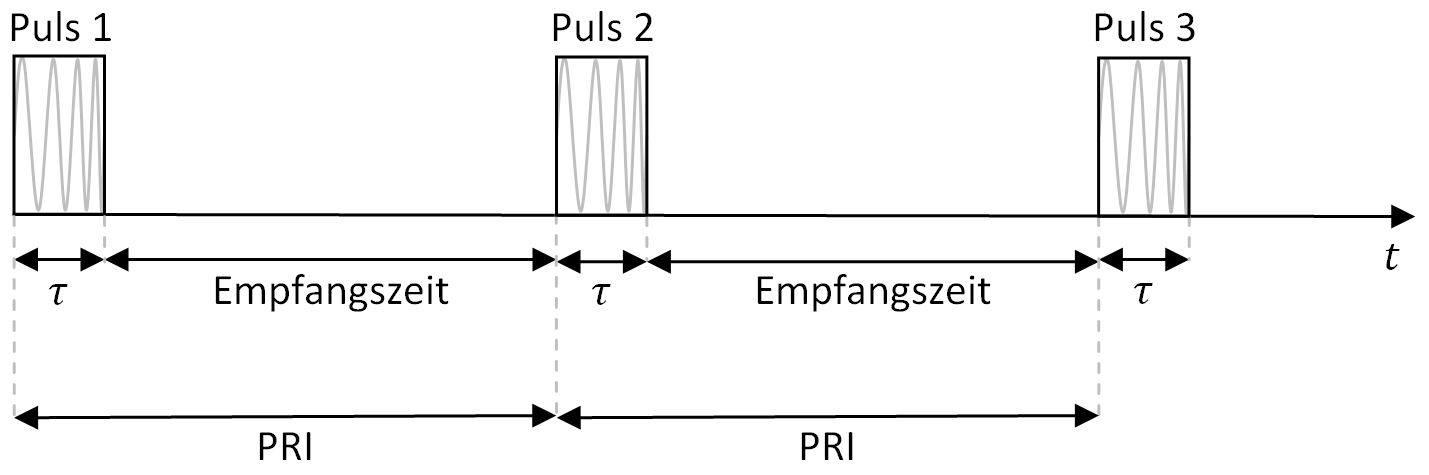
\includegraphics[scale=0.4]{images/Pulse_Radar_PRI_Zoom240.PNG}
  \caption{Schematische Darstellung von mehreren PRIs im Zeitbereich}
  \label{fig:PRI}
\end{figure} 
%


